\label{sec:intro}

With the the development of hardwares and algorithms, the intellegence of a single agent has been greatly improved in recent years. 
The cooperation of agents can expand the capability of a unmanned system, and the multi-agent intelligent system is a promising research field.

Multi-robot exploration (MR-Explore), which provides the location and map for each robot, is the basic task of many multi-robot applications, such as multi-agent navigation and multi-agent rescue. 
For the keyword \textit{"robot"}, the feature-point extraction (FE) is a basic component for the visual odometry to estimate the 6 degree of freedom (6-DoF) pose.
For the keyword \textit{"multi"}, decentralized place recognition (PR), which translates an input image to a short representation code, is a fundamental element to produce candidate place matches.
Previous works use CNN to extract feature-points \cite{detone2018superpoint, simo2015discriminative, yi2016lift} and generate the representation code \cite{arandjelovic2016netvlad, radenovic2018fine}. The CNN-based feature-points from \cite{detone2018superpoint} reaches 10\%-30\% higher matching accuracy compared with the popular hand-crafted extraction method, ORB \cite{Mur-Artal:2017281}. The accuracy representation code from CNN-based method \cite{radenovic2018fine} is also ??\% better than the hand-crafted method [??].

\begin{figure}
	\centering
	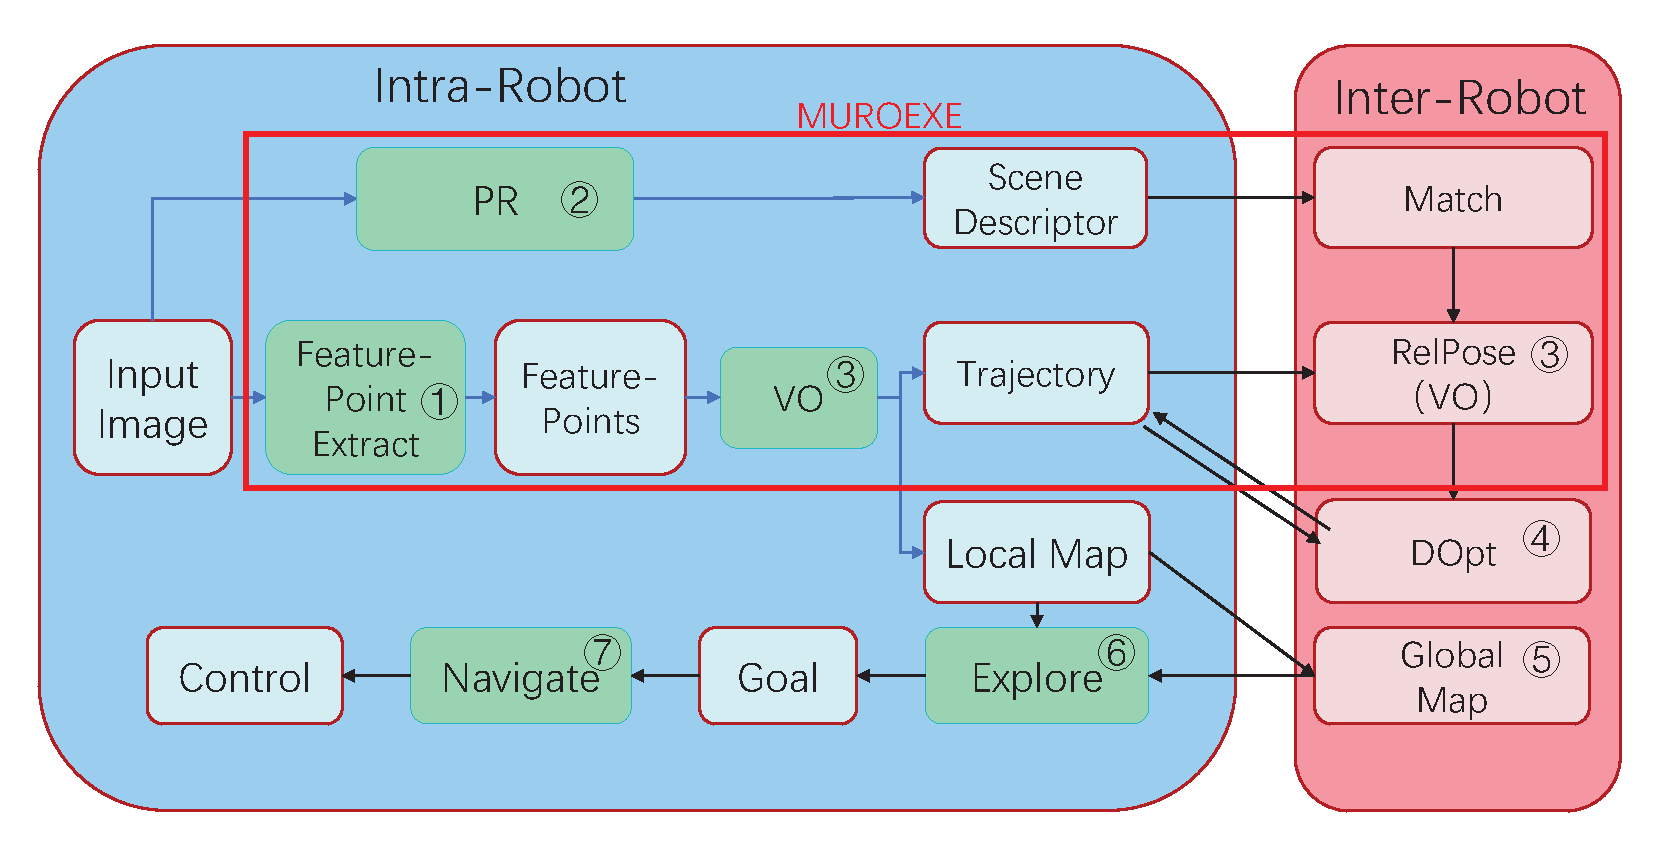
\includegraphics[width=0.99\linewidth]{fig/maexp.eps}
    \caption{
        The modules in MR-Explore. \textcircled{1}\textcircled{3} are basic for a single robot, should be execute every frame. \textcircled{2} generates representation code for some key frames. \textcircled{7}\textcircled{8} are only executed when representation codes are matched across robots and they are latency tolerant.  \textcircled{4}\textcircled{5}\textcircled{6} are for decision and navigation, also latency tolerant.
    }
	\label{fig:maexp}
\end{figure}

\Cref{fig:maexp} illustrates the computation modules in MR-Explore. Feature-point extraction (\textcircled{1}) and visual odometry (VO, \textcircled{3}) should be executed for each input frame, and should be finished before next frame. 
Place Recognition (PR, \textcircled{2}) generates representation code for some key frames, and sends the representation code to other robots. 
When the  representation codes from different robots are matched, optimizaion (\textcircled{7}) can map merging ((\textcircled{8})) are executed to merge the trajectories and maps. \textcircled{4}\textcircled{5}\textcircled{6} are for decision and navigation based on the merged maps. 
The Feature-point extraction (\textcircled{1}) and  Place Recognition (\textcircled{2}) steps are implemented in CNN methods in this paper.
Besides these two modules, some more CNN-based methods, such as semantic segmentation \cite{long2015fully} and object detection \cite{ren2015faster}, can also be introduced to embedded moving robots for better accuracy.
Even if only FE and PR are implemented in CNN, the computational complexity reaches 1 TOP/s , which poses a challenge for embedded systems.

To accelerate CNN on FPGA, some previous works design frameworks to generate a specific hardware architecture for a target CNN, based on  RTL \cite{li_high_2016} or HLS \cite{lu_evaluating_2017}. These works need to reconfigure the FPGA when running another CNN, and do not support fast switching between different CNNs. Some other works design instruction-driven accelerators \cite{yu2018instruction,qiu2016going}, making fast switching possible by providing different instruction sequences. However, previous instruction-driven CNN accelerators need to schedule the entire CNN, which can not automatically schedule two or more tasks simultaneously. The unsupportability of multi-task of CNN accelerator makes it difficult for researchers on robot to use embedded FPGA.


\begin{figure}
	\centering
	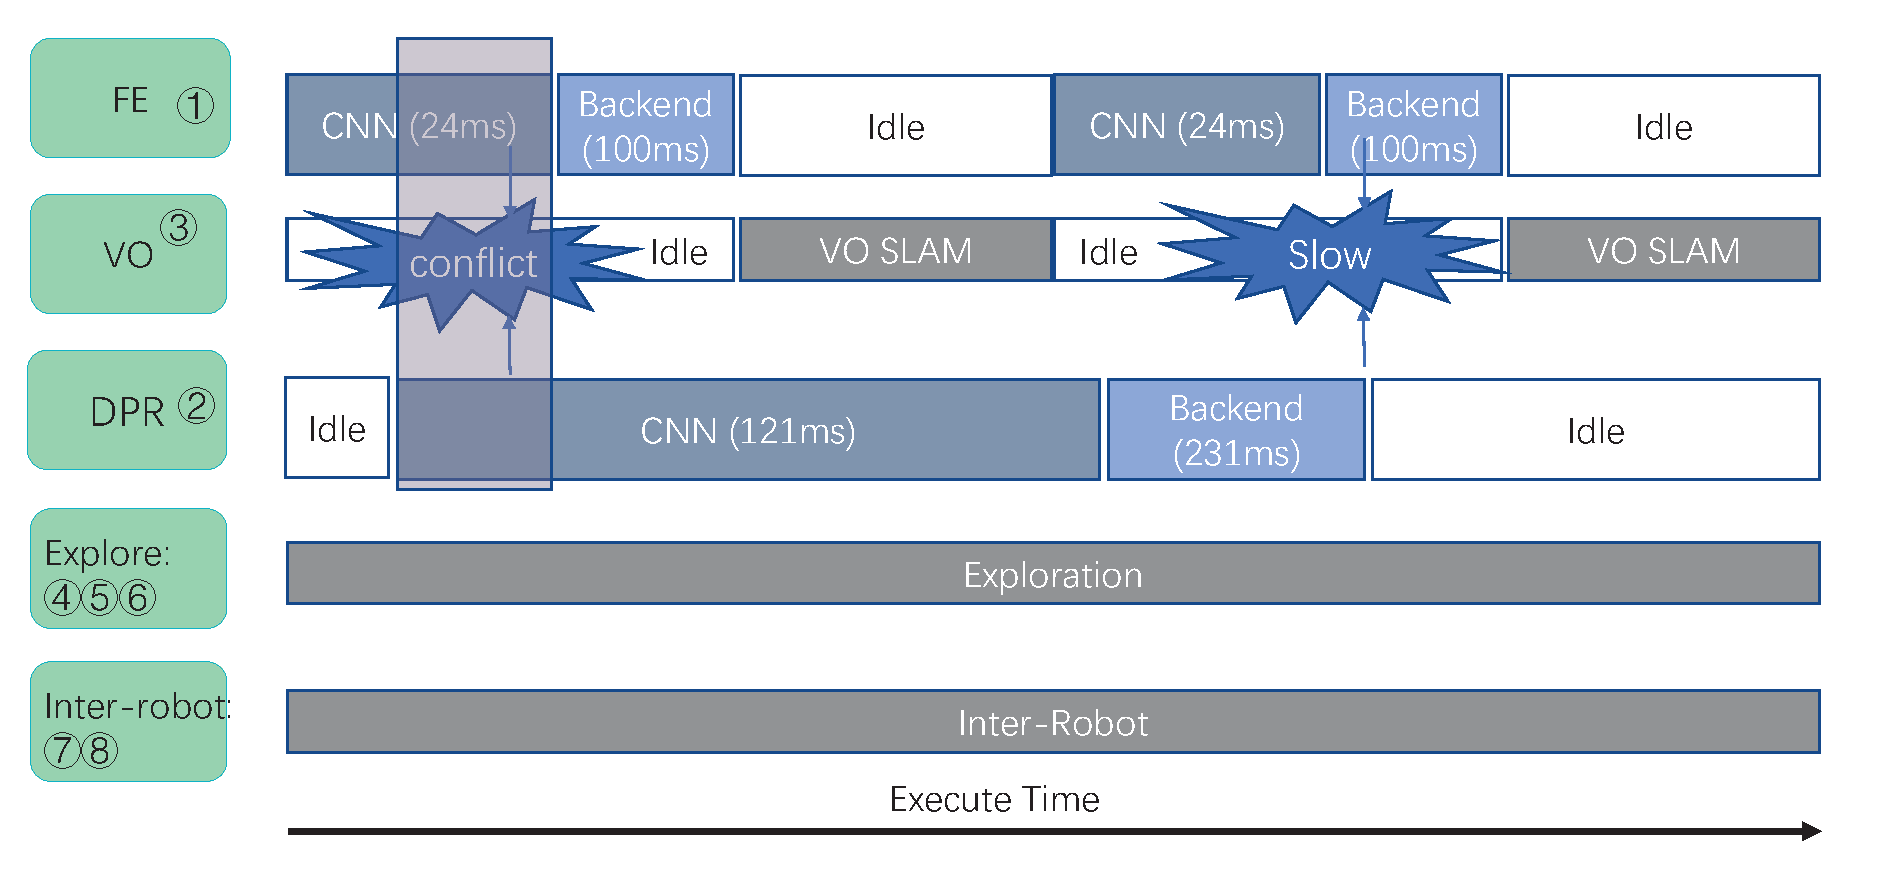
\includegraphics[width=0.99\linewidth]{fig/overalltime.eps}
    \caption{
    The overall timeline of MA-Explore.
    }
	\label{fig:overalltime}
\end{figure}

The overall timeline of MA-Explore is illustrated in \Cref{fig:overalltime}. The threads of FE and PR may need to process CNN at the same time, leading to hardware resouces conflicts. To make the researchers on robot easy to use FPGA, the accelerators should support the following features.

\textbf{Multi-thread:} A robot contains many modules including perception, decision and control. The Robot Operating System (ROS) \cite{quigley2009ros} is a popular middleware fusing different modules from different developers. In ROS, each module is considered as an indepentant thread on CPU. The FPGA accelerators should be easily accessed by different threads.

\textbf{Dynamic Scheduling:} The execution of CNN is depend on other operations, like VO module in \Cref{fig:overalltime}. These operations are running at CPU, and the execution time varies with the input data (10ms - 50ms for VO). The accelerators cannot predict when to start a task. The FPGA accelerators should be scheduled dynamically to support irregular task requests from the software.

\textbf{Scheduling by priority:} Each module has different priority, the control and perception tasks usually have higher priority, and the priority of long-term decision and optimization is lower \cite{RamsauerKLM17}. The FPGA accelerators need to schedule the critical tasks first.

Besides the CNN backbone, the post-processing of the CNN-based methods are also computation consuming. As illustrated in \Cref{fig:overalltime}, the execution time of post-processing on embedded CPU (~100ms) exceeds that of CNN backbone (30ms) on the accelerator, becoming the bottleneck.


To make the CNN accelerator flexible enough for researchers on robot and the post-processing of CNN-based method executed in real time, we propose a \textit{MU}lti-\textit{RO}bot \textit{EX}ploration \textit{E}ngine ( MUROEXE ) to deploy the MR-Explore on embeded FPGA, with following contributions:

\begin{itemize}
    \item We propose a CNN-based MA-Explore framework based on FPGA. The modules in MUROEXE is designed for ROS \cite{quigley2009ros}, so that the modules can be easily used in other applications.
    \item We propose a \textbf{Virtual Instrcution Interruption} method, making the CNN accelerator support dynamic multi-thead scheduling by priority.
    \item We optimize the data flow of the post-processing operations. RTL/HLS modules are designed for the optimized post-processing.
\end{itemize}

The rest of this article is organized as follows: \Cref{sec:relate} will introduce the related work. \Cref{sec:cnninterrupt} details the virtual instruction interruption. \Cref{sec:hardsoftcodesign} optimizes the post-processing. \Cref{sec:muroexe} introduce the MUROEXE framework with ROS. Experimental results and analysis are given in \Cref{sec:experiments}. \Cref{sec:conclusion} concludes this article.